\chapter{Architecture}
\label{chapter:architecture}
%Esta secção deve englobar:

%\begin{itemize}
%    \item Uma análise de requisitos, onde devem “abrir” portas para as principais
%        características da vossa arquitectura.
%    \item Uma descrição de alto nível da arquitectura do vosso sistema. Esta descrição
%        pode ser:
%        \begin{itemize}
%            \item A arquitectura de rede, explicando os principais componentes e as
%                funções que executam.
%            \item A arquitectura de SW da aplicação, explicando os principais
%                componentes e as funções que executam.
%        \end{itemize}
%    \item Descrições detalhadas de todos os componentes da vossa arquitectura.
%    \item As escolhas que efectuarem em termos de arquitectura global e de detalhe,
%        devem ser justificadas, face aos requisitos que identificaram.
%\end{itemize}

%Sempre que possível, ilustrem a arquitectura com figuras, que descrevam
%sucintamente o modelo como na Figure~\ref{fig:logoCNM}.

%\begin{figure}[!htb]
%  \centering
%  \includegraphics[width=0.25\textwidth]{Figures/logoCNM.png}
%  \caption[Caption for figure in TOC]{Caption for figure.}
%  \label{fig:logoCNM}
%\end{figure}

Taking into account the goals of this project and all the technology presented so far. Our proposal is the development of a web application that provides communication and collaboration features in real-time.

The requirements for our web application are:

\begin{itemize}
 \item Text, Audio and Video communication using \ac{WebRTC}.
 \item Ability to record and playback interactive multimedia.
 \item Create annotations over video and voice content.
 \item Enrich communications by overlaying multiple media types.
 \item Search and navigate through annotations and contents.
 \item Ability to create and share time links among users.
 \item Mix multiple user streams into a single stream.
 \item Sound detection for showing the current speaker.
 \item Structure presentation of the content.
 \item Collaborative text edition.
 \item Easy interface for content creation and synchronization. 
\end{itemize}

	Moreover we allow clients to discover chat rooms and other clients by navigating on the web pages provided by our web server. In addition users can create rooms for multi-party audio and video communication communication which is achieved by using \ac{WebRTC}'s \emph{MediaStream} and \emph{PeerConnection}.

	Furthermore, chat rooms can be public or private. Public chat rooms are moderated by a group of clients which initially is only the room creator, this type of room has no access restrictions by default, but that can be changed by its moderators. Private chat rooms will be visible for a defined list of clients or can be accessed by clients that have a link for that conference room.

\section{Modules}

	In this section we present the modules of our application.

\begin{figure}[!htb]
	\centering
	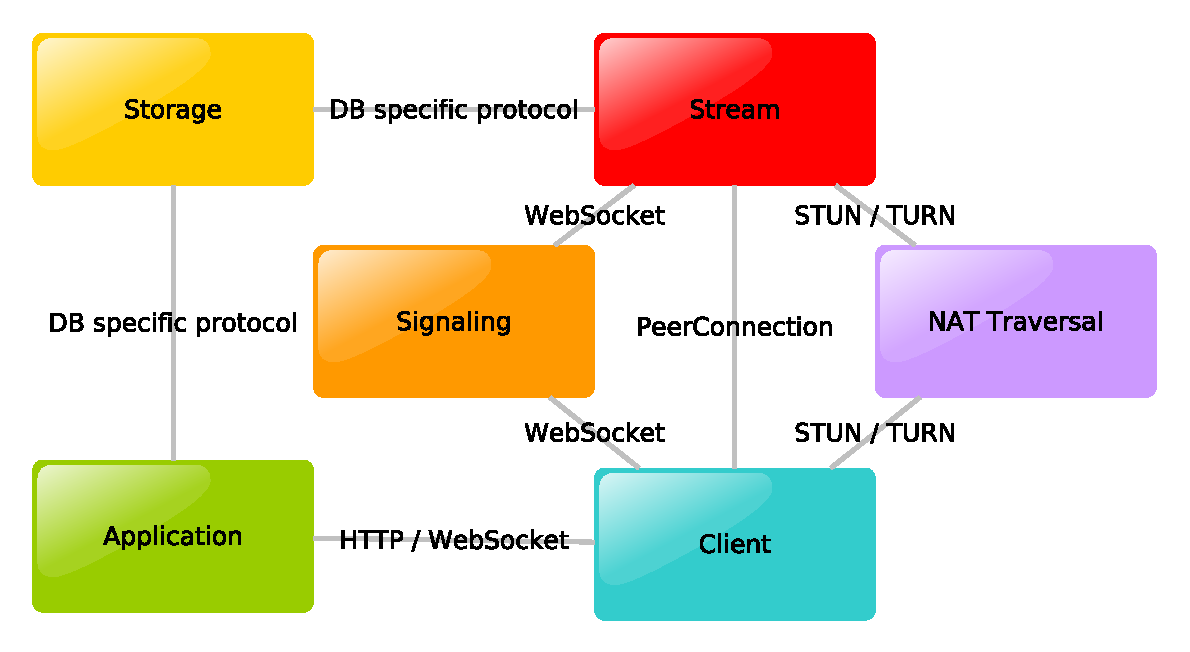
\includegraphics[width=0.8\textwidth]{figures/modules.pdf}
	\caption{System Modules}
        \label{fig:modules}
\end{figure}
%RP as figuras têm de ser apresentadas. Figure~\ref{fig:modules} presents ...
	Figure~\ref{fig:modules} presents the structure of our system which is divided into six modules:

\begin{itemize}

\item \underline{Application module} - responsible to provide information about the relevant modules (\emph{NAT Traversal} and \emph{Signaling}) and user interface to the \emph{Client}.

\item \underline{Signaling module} - responsible for \emph{Client} and \emph{Stream} coordination.

 \item \underline{NAT Traversal module} - used by \emph{Client} and \emph{Stream} modules during the \emph{Signaling} phase which ends by establishing the connection between them.

 \item \underline{Stream module} - responsible to deliver and receive multimedia content from the \emph{Client}. 

 \item \underline{Storage module} - responsible store all the model information and media recorded. 

 \item \underline{Client module} - responsible for the interaction with the user.

\end{itemize}



% Each room will be associated to multiple Media-Types, interactive and non-interactive, discrete and continuous. This media types can be structured with chains of events. Some components of the user interface may not be synchronized to all participants, for example an help or suggestion window.  

 
\section{Implementation Proposal}
The infrastructure is composed by: web server, stream server, signaling server, database and video repository.



\begin{figure}[H]
	\centering
	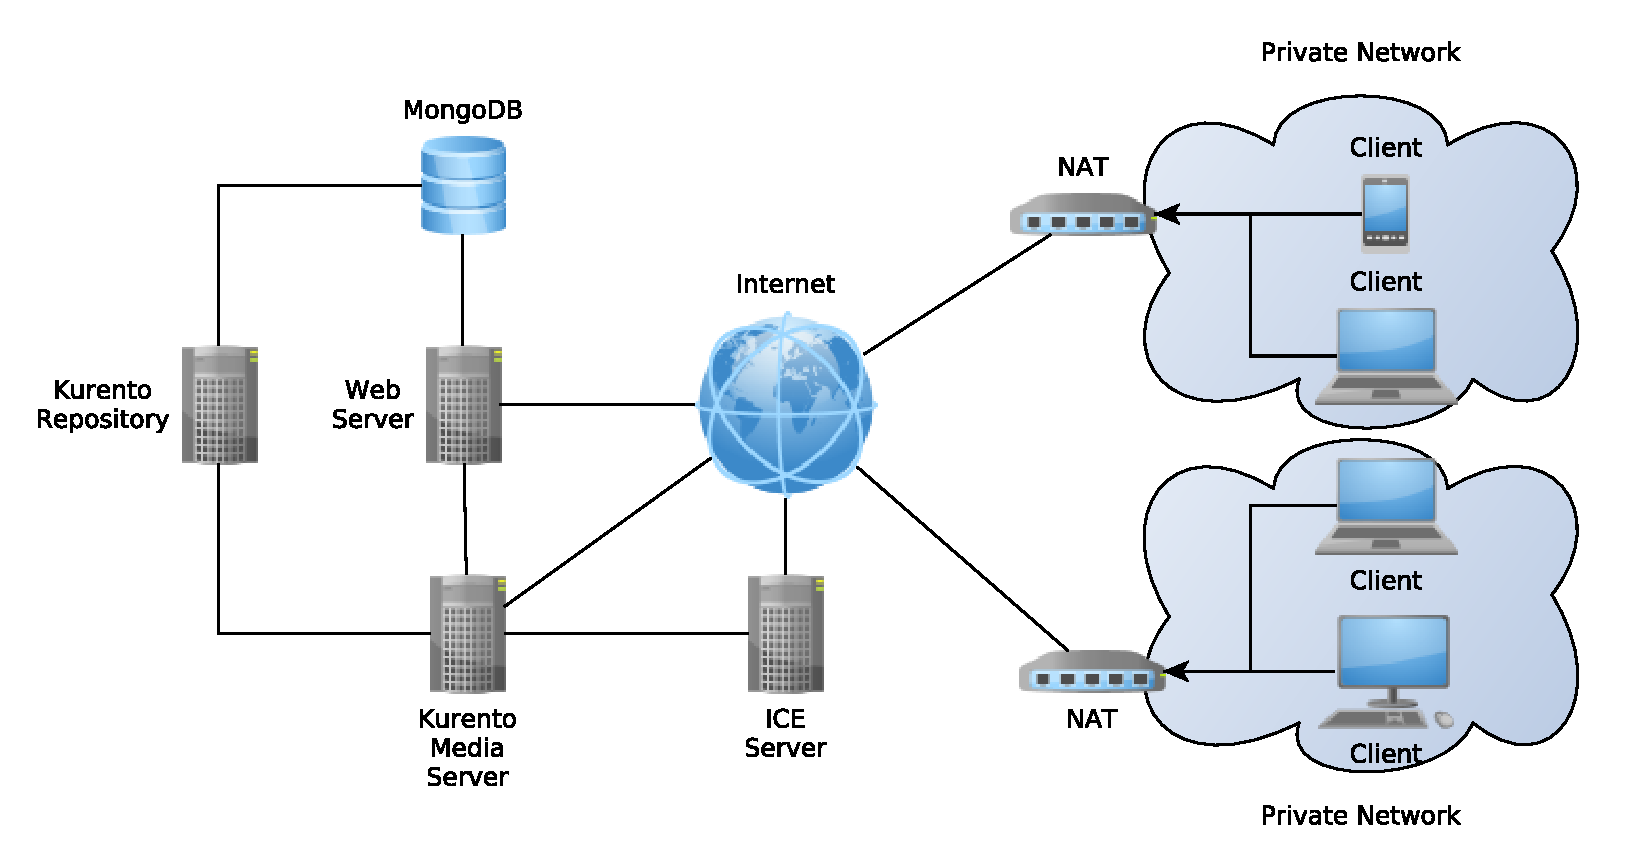
\includegraphics[width=\textwidth]{figures/infrastructure.pdf}
	\caption{System Infrastructure}
\end{figure}

In order to simplify our solution, we propose both the \emph{Application}, \emph{Signaling}, \emph{Stream} and \emph{Storage} modules implementation within the same server application so it could be easy to deploy as a single image. To this set of modules we often call \emph{backend}.

Having established that the \emph{backend} modules are placed in the same machine, that helps controlling which resources the client has permission to access as those modules are seen as a private network.

To qualify the above we provide public access to \ac{HTTP} server ports, maintaining the access to other components restricted through firewall rules. In relation to the database there is no directly access from outside, all the database information is accessed via our application server which validates the permissions of users when acting above our system.

On the other hand, the access to our streaming servers is also restricted but clients can connect to them after concluding the signaling phase. This signaling phase may or not proceed in function of the client access permissions, for example if a user is trying to access a private conference room that is not member of or has no invitation link, the signaling server rejects to start the signaling phase and the user cannot access to the streaming server.

Furthermore, we have taken into account the compatibility between the streaming server, database and the operation transformation solutions in order choose the appropriate framework to implement our web server.

As a result of our study about signaling protocols we have decided to exclude \ac{XMPP} due to the development difficulties that it exposes when using multiple web pages, namely the user re-authentication performed each time a page is loaded and the single tab usage limitation. By consequence we have not chosen \emph{Jitsi Video Brigde} as it uses \ac{XMPP}.

Accordingly, by excluding \emph{Jitsi Video Brigde} we have decided that our solution must use \ac{KMS}. Our web server could be implemented easily with \emph{NodeJS} or \emph{Java} due to the fact \ac{KMS} provides clients for both technologies but others could be used as \ac{KMS} also exposes their \ac{API} via \emph{WebSockets}.

By default, \emph{Kurento Repository} is implemented over \emph{MongoDB}, for convenience our storage model will also use the same database. 

Due to the fact we are going to use \ac{KMS} as streaming server solution, we could choose \emph{NodeJS} or any \emph{Java} based web framework for implementing our web application server. One of our criteria for choosing the web framework is the ability to follow the \ac{MVC} paradigm which can help us to organize our code. Without any strong reason we have decided to implement our web server with \emph{PlayFramework}\footnote{\url{https://www.playframework.com/}(acessed March 25, 2016)} using \emph{Java}.

Importantly, for the collaborative text editor, we have chosen \emph{OT.js} due to its server and storage implementation choice independence.

For the \emph{NAT Traversal} module an \ac{ICE} server is not required to be on our infrastructure, as a public \ac{STUN} server can be used for testing our solution although we recognize that for a production environment we would need to maintain our own \ac{TURN} servers in order to ensure connectivity to all clients.

Not less important, on the client computers, both \emph{Mozilla Firefox} and \emph{Google Chrome} should be installed as web browsers. Libraries such as \emph{jQuery}, \emph{Bootstrap}, \emph{Adapter.js}, \emph{OT.js} can be downloaded from the web server and executed on the client side.

\begin{table}[H]
\centering
	\caption{Application Architecture}
	\label{table:apparch}
    \begin{tabular}{cccccccc@{}m{0pt}@{}}
	\hline 
\multicolumn{8}{|c|}{\cellcolor{Gray}Application}  &\\[12pt]\cline{1-5}\cline{7-7}
\multicolumn{1}{|c|}{jQuery} & \multicolumn{1}{c|}{HTML5} & \multicolumn{1}{c|}{CSS3} & \multicolumn{1}{c|}{Signaling} & \multicolumn{1}{c|}{~~~~~ot.js~~~~~} & \multicolumn{1}{c|}{\cellcolor{Gray}~~~~~~~~~~~~~~~} & \multicolumn{1}{c|}{adapter.js} &   \multicolumn{1}{c|}{\cellcolor{Gray}~~~~~~~~~~~~~~~} &\\[12pt]\hline
\multicolumn{1}{|c|}{HTTP} & \multicolumn{2}{c|}{User Interface}  & \multicolumn{3}{c|}{WebSocket}    & \multicolumn{2}{c|}{WebRTC}      &\\[12pt]\hline
\end{tabular}
\end{table}

Table~\ref{table:apparch} presents the application architecture and the underlying technologies seen from the user's perspective. \emph{Adapter.js} and \emph{jQuery} will ensure that our application is compatible with the most popular web browsers.
\emph{Bootstrap} will be used to make the user interface more appellative and responsive. With \emph{Bootstrap} it is quite easy to develop applications that adapt to mobile devices with different screen sizes.

The synchronization between multimedia elements will be performed trough chains of \emph{JavasSript} events or by specifying the interval of time which time content must be visible. Other animations can be implemented with \ac{SVG} embedded on \ac{HTML}.

\section{Chapter Summary}
\label{architecture:summary}

In this chapter we have shown the modules needed in order to implement our solution.

Several technologies were taken into account for implementing each module, we have studied the pros and cons of each technology and decided the architecture for our solution.

